% PLEASE USE THIS FILE AS A TEMPLATE
% Check file iosart2x.tex for more examples

% add. options: [seceqn,secthm,crcready,onecolumn]
\documentclass[sw]{iosart2x}
\usepackage{hyperref}
%\usepackage{dcolumn}
%\usepackage{endnotes}

%%%%%%%%%%% Put your definitions here


%%%%%%%%%%% End of definitions

\pubyear{0000}
\volume{0}
\firstpage{1}
\lastpage{1}

\begin{document}

\begin{frontmatter}

%\pretitle{}
\title{Searching the optimal fragment: managing real-time and historical data with Linked Connections}
\runningtitle{Article Title}
%\subtitle{}

% For one author:
%\author{\inits{N.}\fnms{Name1} \snm{Surname1}\ead[label=e1]{first@somewhere.com}}
%\address{Department first, \orgname{University or Company name},
%Abbreviate US states, \cny{Country}\printead[presep={\\}]{e1}}
%\runningauthor{N. Surname1}

% Two or more authors:
\author[A]{\inits{D.}\fnms{David} \snm{Chaves-Fraga}\ead[label=e1]{dchaves@fi.upm.es}},
\author[B]{\inits{J.}\fnms{Julian} \snm{Rojas}\ead[label=e2]{julianandres.rojasmelendez@ugent.be}},
\author[B]{\inits{P.}\fnms{Pieter} \snm{Colpaert}\ead[label=e3]{pieter.colpaert@ugent.be}}
\author[A]{\inits{O.}\fnms{Oscar} \snm{Corcho}\ead[label=e4]{ocorcho@fi.upm.es}}
and
\author[B]{\inits{P.}\fnms{Ruben} \snm{Verborgh}\ead[label=e5]{ruben.verborgh@ugent.be}}
\runningauthor{Chaves-Fraga et al.}
\address[A]{Ontology Engineering Group, \orgname{Universidad Polit\'ecnica de Madrid}, \cny{Spain}}
\address[B]{IDLab, Department of Electronics and Information Systems, \orgname{Ghent University-imec}, \cny{Belgium}
\printead[presep={\\}]{e1,e2,e3,e4,e5}}

%\begin{review}{editor}
%\reviewer{\fnms{First} \snm{Editor}\address{\orgname{University or Company name}, \cny{Country}}}
%\reviewer{\fnms{Second} \snm{Editor}\address{\orgname{First University or Company name}, \cny{Country}
%    and \orgname{Second University or Company name}, \cny{Country}}}
%\end{review}
%\begin{review}{solicited}
%\reviewer{\fnms{First} \snm{Solicited reviewer}\address{\orgname{University or Company name}, \cny{Country}}}
%\reviewer{\snm{anonymous reviewer}}
%\end{review}
%\begin{review}{open}
%\reviewer{\fnms{First} \snm{Open Reviewer}\address{\orgname{University or Company name}, \cny{Country}}}
%\end{review}

\begin{abstract}
Deal with the access and the management of static, but also historical and real-time data, is one of the most relevant problems in several domains which want to take advantage of the benefits of Linked Data. The transport domain is one of these domains but, nowadays, their data are exposing in a way that only ad-hoc systems are able to process them. In previous work, the Linked Connections (LC) framework was introduced as a cost-efficient publishing alternative to the \textit{de-facto} GTFS standard and route planning APIs. At the moment that the route planners take into account real-time and historic data, new issues appear, like for example how we should expose the data on the web, how to improve the query performance or how to ensuring data consistence.

In this paper we present the advances made in the LC framework to deal with real-time and historical data in the transport domain providing a light HTTP interface that allows smart clients to create their own route planners. Our main contribution is a LC server, based on the principles of Linked Data Fragments, that is able to specify the size of each fragment, improving the query evaluation performance and providing a robust access to the data. We also implement the memento protocol in the top of LC and create a new metadata model for improving the discoverability of transport datasets. We evaluate and compare our approach with other possibilities that are also able to deal with real time and historic data. We discover that take into account the size of the fragments has a relevant impact in the performance on the route planning algorithms.  
\end{abstract}

\begin{keyword}
\kwd{Linked Connections}
\kwd{Historical Data}
\kwd{Real time data}
\end{keyword}

\end{frontmatter}

%%%%%%%%%%% The article body starts:

%\section{}\label{s1}

%\subsection{}\label{s1.1}
\section{Introduction}\label{introduction} %Oscar and David
In the current state of the Web of Data, a wide amount of that data are exposed following the principles of Linked Data. Giving unique identifiers to each resource, representing the data using a shared and common vocabulary of the domain or the possibility of \textit{dereferencing} each URI are some of the relevant aspects that made Linked Data as one the most relevant approaches to organize and expose the data on the Web. Other benefit that is also important is the opportunity of querying Linked Data following approaches like SPARQL or APIs. However, due to this last benefit a lot of several issues in terms of performance at the moment that complex data and queries are involved. One relevant issue is how to deal with different data sources that provide information about multiple features of the same service. For example, in the case of transport route planning, several versions of the same dataset and its integration with a real-time service, creates an environment where developing solutions able to integrate, manage and query that data in a robust way is very important to improve the current informational services.


Currently, the information services from several domains (like transport) are not able to deal with the heterogeneity of the vocabularies and the formats so they provide ad-hoc solutions. A decentralized solution that carries the possibility for the companies to raise the dataset for a semantic interoperability level is needed. In the past, the Linked Connections\cite{colpaert2015intermodal} framework provided a efficient cost HTTP interface to exploit the implicit information of the standard \textit{de-facto} for static transport data, GTFS\footnote{\url{https://developers.google.com/transit/gtfs/}}. However, the companies have started to provide access to their real-time data so it is important to take into account this information to improve the quality of experience of the passengers and the mobility in the cities where the contamination is a big healthcare problem. In terms of data management, there are two relevant problems that should be solved. On one hand, the interoperability between the different data sources and standards that represent the domain and provide a solution that easy adapts to different requirements of each company, which is one of the main contributions of LC. On the other hand, take into account historical and real-time data in route planning will improve the quality of the information for the passengers but the amount of data increases as time passes so a solution that expose the data integrating several 

Since May 2017, one of the main motivations for developing solutions about multimodal and integrated travel information services is the publication of the new directive by the EU Comission about discoverability and access to public transport data across Europe. This document proposes the making of public transport data from providers available on national or common access points saved on databases, data warehouse or repositories. All the states will provide access to a unique common point following different standards that the directive allow as Transmodel, Datex II or GTFS. So a solution able to deal with the heterogeneity of access points and data formats and it also provides an approach to efficiently query them is necessary.

Linked Data Fragments (LDF) propose a simply but efficient way to move the load of the triple-based servers to the client side improving the server availability. Following this approach, the Linked Connections (LC) framework applies the bases of LDF to provide an efficient HTTP interface for the transport domain. But at this moment, any common solution is able to integrate and expose real-time and historical data in a way that the performance does not influence the user experience of the informational services. In this paper we present the advances we carry out on the Linked Connections (LC) framework, focused on dealing with real-time and historical data. The main contribution is providing a solution that is able to expose transport data on the Web in an optimal way for improving the querying performance. One the requirements for route planning is to sort the data depending on the time so until now, LC exposed the data in multiple fragments depending on that variable, so the size of each fragment depends of the number of connections for a specific time. It affects to the querying performance because the solution is affected by the heterogeneity of the fragments size. The advances in the LC framework allow to query the data without the necessity of splitting them based on time variable, providing a more homogeneous scenario, integrating static, real-time and historical data and improving the performance of the query evaluation as we show in the Section 5. Our approach wants to set the bases for dealing with the heterogeneity of the domain that will appear in the following years based on the proposal of the EU Comission.

The paper is organized as follows: Section 2 presents some of the related work on benefits of Linked Data, solutions to query data on the web, the EU regulation about the availability of transport data on the web and current (semantic) route planners. Section 3 describes our proposal about the improvements of the Linked Connections framework. Section 4 presents the design of our experiments. Section 5 describes the results we obtained evaluating our main contributions. Section 6 provides a brief discussion about the relevance of our contributions, and Section 7 presents conclusions and areas for future work.


\section{Related Work}\label{related_work} %David
On the current state of the Web, huge amount of data are exposed following the principles of Linked Data. We describe the main contributions on this topic, and also the relevance of the ones made in querying data on the web and the current solutions on planning transport routes using semantics.

\subsection{Linked Data}
%what is linked data and its benefits
One of the most well-known alternatives to publish data on the Web is Linked Data \cite{bizer2009linked}. Linked Data allows to identify in an unique way resources on the Web using identifiers, or HTTP URIs. It is a method to distribute and scale data over large organizations such as the Web. When looking up this identifier by using the HTTP protocol or using a Web browser, a definition must be returned, including links towards potential other interesting resources, a practice called \textit{dereferencing}. The triple format to be used in combination with URIs is standardized within RDF. The URIs used for these triples already existed in other data sources, and we thus favored using the same identifiers. It is up to a data publisher to make a choice on which data sources can provide the identifiers for a certain type of entities. 

There are multiple benefits of exposing the data on the Web as Linked data: i) the data is linked to related data so the information can be combined across different interfaces, ii) the data is queryable using the query language for RDF, SPARQL \cite{prud2006sparql}, or other approaches like API-Rest interfaces \cite{world2014json} or \cite{lanthaler2013creating} iii) the data is represented following a reference model, so the interoperability between different data sources is at the semantic level.

\subsection{EU directive in multimodal transport services}

\subsection{Querying data on the Web}

\subsection{Route planning}



\section{Linked Connections}

\subsection{Linked Connections server}

\subsection{The memento protocol}

\subsection{Route planning algorithms}

\section{Evaluation Design}


\begin{figure}[t]
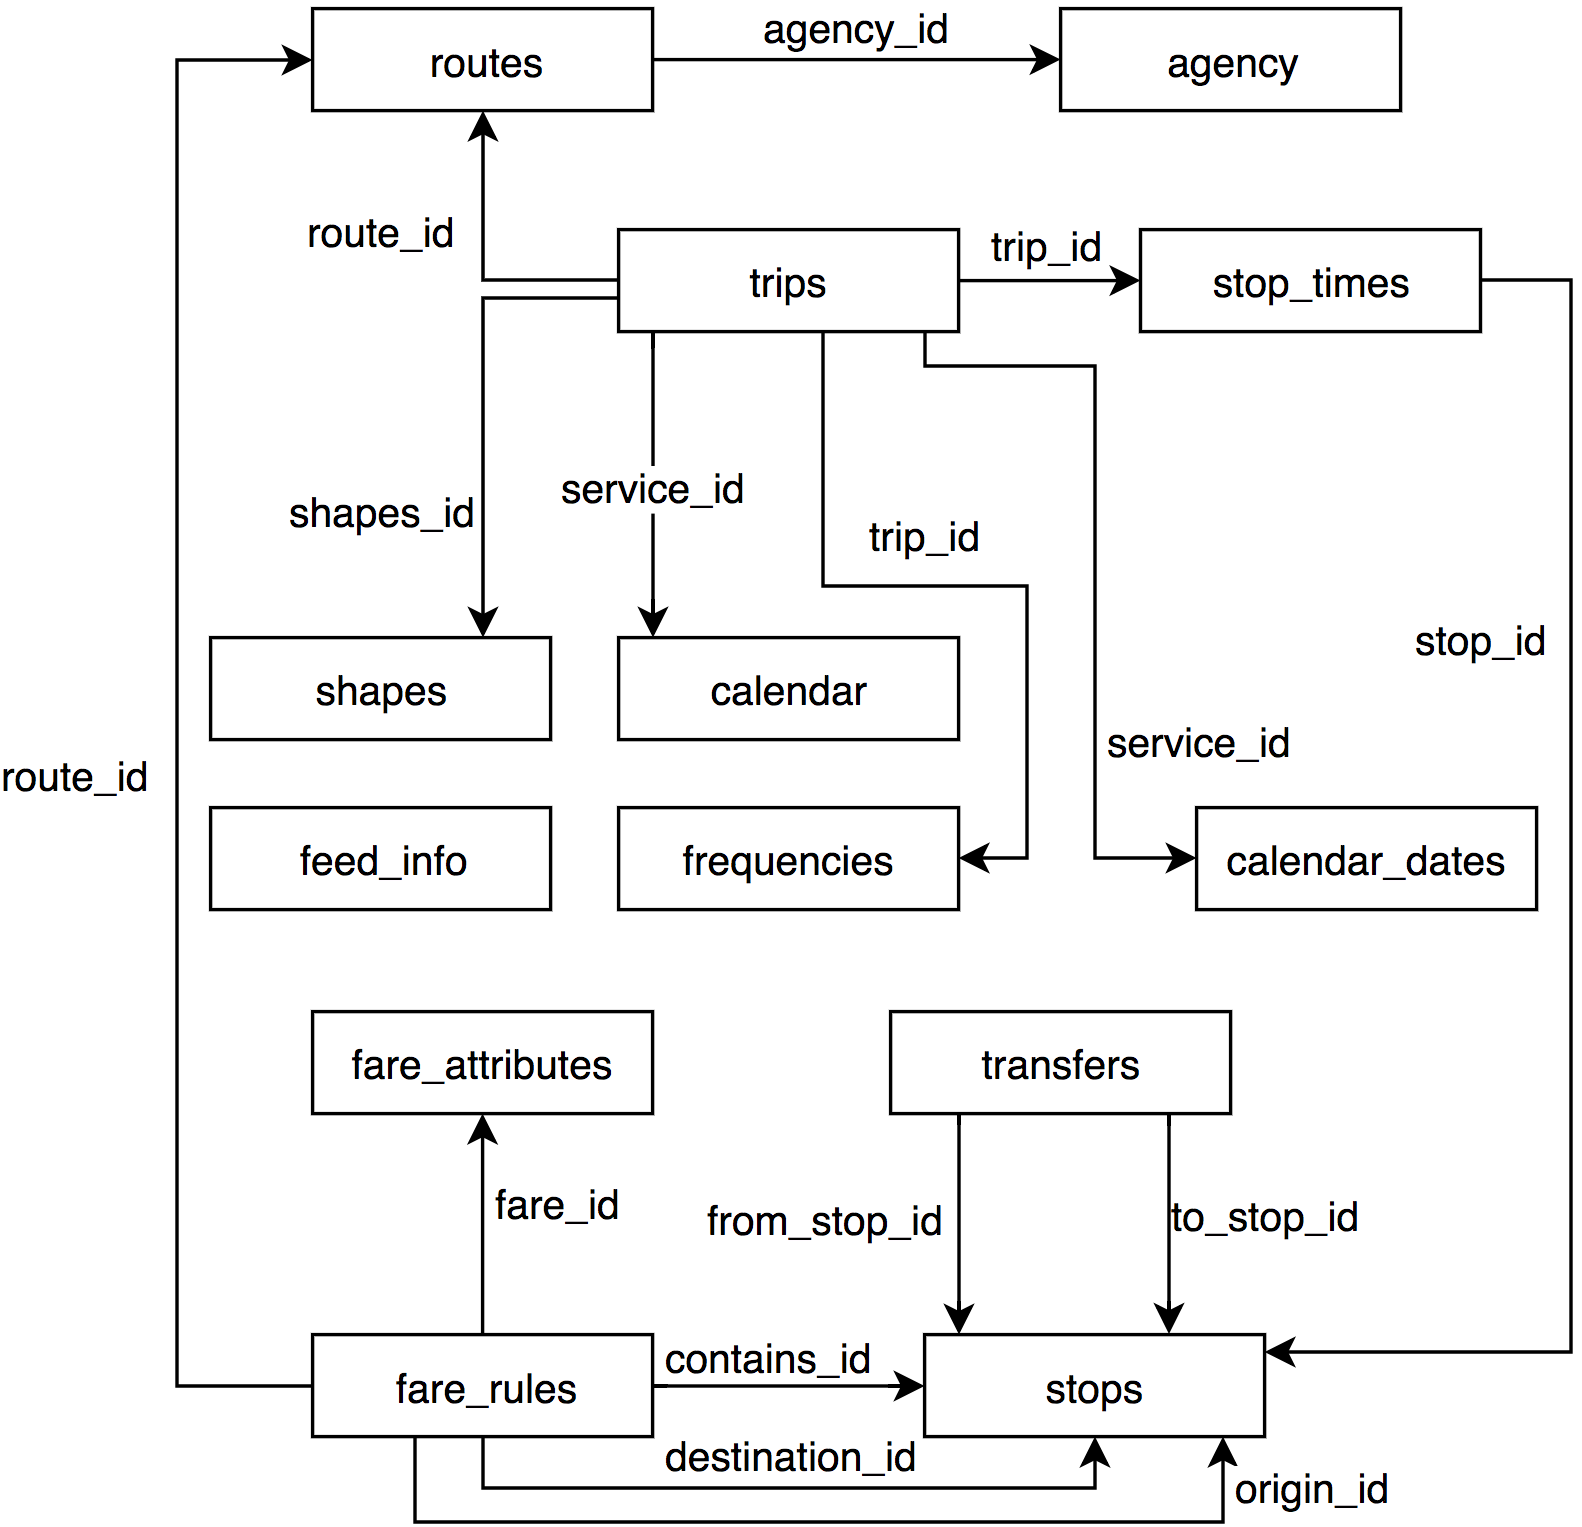
\includegraphics[width=0.4\textwidth]{images/gtfsmodel.png}
\caption{Figure caption.}\label{f1}
\end{figure}

\begin{figure}[t]
	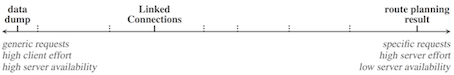
\includegraphics[width=0.45\textwidth]{images/lc.png}
	\caption{Figure caption.}\label{f2}
\end{figure}

\section{Results}

\section{Discussion}

\section{Conclusions and Future work}

\begin{acks}
	
\end{acks}

%\begin{figure}[t]
%\includegraphics{}
%\caption{Figure caption.}\label{f1}
%\end{figure}

%\begin{table*}
%\caption{} \label{t1}
%\begin{tabular}{lll}
%\hline
%&&\\
%&&\\
%\hline
%\end{tabular}
%\end{table*}

%%%%%%%%%%% The bibliography starts:

%%%%%%%%%%%%%%%%%%%%%%%%%%%%%%%%%%%%%%%%%%%%%%%%%%%%%%%%%%%%%
%%                  The Bibliography                       %%
%%                                                         %%
%%  ios1.bst will be used to                               %%
%%  create a .BBL file for submission.                     %%
%%                                                         %%
%%                                                         %%
%%  Note that the displayed Bibliography will not          %%
%%  necessarily be rendered by Latex exactly as specified  %%
%%  in the online Instructions for Authors.                %%
%%                                                         %%
%%%%%%%%%%%%%%%%%%%%%%%%%%%%%%%%%%%%%%%%%%%%%%%%%%%%%%%%%%%%%


\nocite{*}
% if your bibliography is in bibtex format, use those commands:
\bibliographystyle{ios1}           % Style BST file.
\bibliography{bibliography}        % Bibliography file (usually '*.bib')

% or include bibliography directly:
%\begin{thebibliography}{0}
%\bibitem{r1} F. Author, Information about cited object.
%
%\bibitem{r2} S. Author and T. Author, Information about cited object.
%\end{thebibliography}

\end{document}
